\vspace{10mm}
\section{Wireframe del sistema}
Ora che tutti i sottosistemi sono stati modellati, è il momento di delineare dei wireframe al fine di ottenere delle linee guida grafiche riguardo quanto specificato fin ora.\newline

\noindent Verranno presentati i wireframe relativi ai due endpoint offerti ai clienti: l'Applicativo di registrazione e l'Applicativo Dashboard.\newline
La piattaforma Atlas di contro non necessita di una GUI in quanto server.\newline

\noindent Per ogni applicativo considerato analizzeremo più wireframe, relativi agli aspetti affrontati nelle sezioni precedenti.
\vspace{50mm}
\subsection{Applicativo di registrazione}
\noindent Il primo wireframe (\emph{figura 2.8}) sintetizza le componenti della {\bf schermata di login}.\newline

\noindent Troviamo le \emph{credenziali} che permettono all'Utente di identificarsi in modo univoco all'interno del sistema: username (identificativo), password e nome dell'organizzazione.\newline

\noindent In fondo è presente il pulsante che permette di effettuare il \emph{login} una volta inserite le credenziali sopra citate.\newline

\noindent Viene inoltre fornita la possibilità di \emph{memorizzare le credenziali} dell'utente.
\vspace{5mm}
\begin{figure}[H]
  \centering
  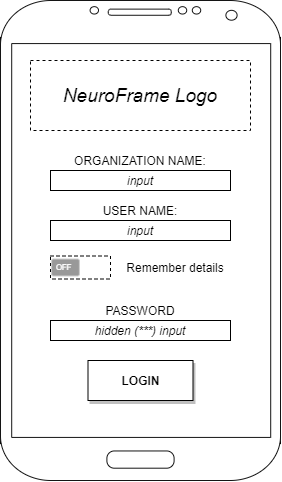
\includegraphics[width=0.4\textwidth]{img/wireframe_app_acquisizione_login.png}
  \caption{Pagina di login dell'Applicativo di registrazione}
\end{figure}
\vspace{5mm}
\noindent Il secondo wireframe invece (\emph{figura 2.9}) contiene {\bf tutte le rimanenti schermate}, sintetizzando un flusso funzionale derivato dall'analisi degli stati (\emph{sezione 2.2.5}).
\begin{figure}[H]
  \centering
  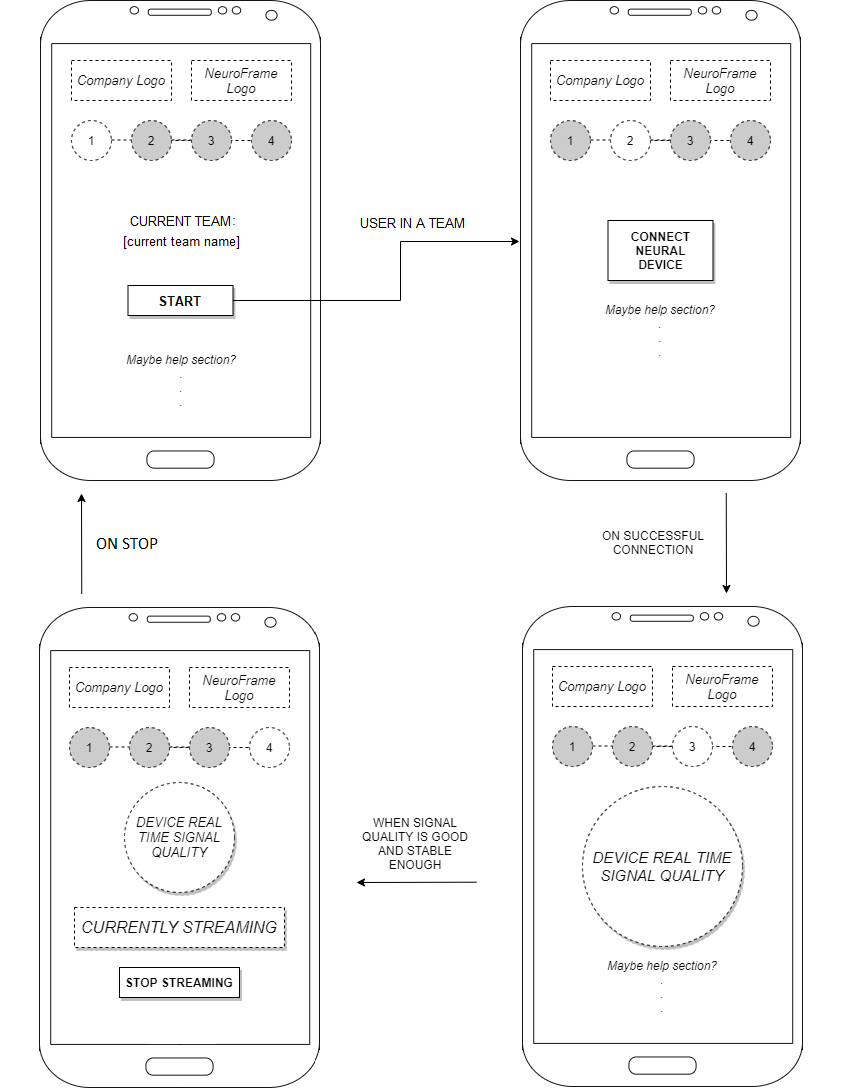
\includegraphics[width=0.65\textwidth]{img/wireframe_app_acquisizione_flusso.png}
  \caption{Flusso funzionale dell'applicativo di registrazione}
\end{figure}
\noindent Nella {\bf schermata 1} l'applicazione attende l'input da parte dell'Utente per cominciare la procedura che porterà allo streaming di dati.\newline
Come da modellazione non è possibile procedere alle prossime fasi fino a che l'Utente non è stato inserito all'interno di un Team da parte di un Team manager (il team corrente viene indicato nella schermata).\newline

\noindent Giunti alla {\bf schermata 2} l'applicativo si trova nuovamente in uno stato di attesa dell'input di un Utente.\newline
Alla pressione del pulsante inizierà la procedura di connessione con il Dispositivo di acquisizione.\newline

\noindent Una volta che la connessione è avvenuta con successo si viene portati alla {\bf schermata 3} dove avviene la stabilizzazione del segnale al termine del quale comparirà la {\bf schermata 4}, mostrando lo streaming in corso e fornendo all'Utente la possibilità di interrompere lo streaming, tornando alla schermata 1.\newline


\subsection{Dashboard}
Sono stati elaborati due wireframe lato applicativo Dashboard: {\bf Login} (\emph{figura 2.10}) e {\bf Dashboard visualizzazione dati} (\emph{figura 2.11}).\newline
Il primo wireframe presenta gli elementi standard di un qualsiasi form di login: un identificativo ed una password.\newline
Si può notare l'\emph{assenza} di due funzionalità di uso comune:
\begin{itemize}
  \item \emph{Registrazione}:
  data la natura di NeuroFrame come servizio in abbonamento alle aziende le credenziali verranno comunicate direttamente all'azienda, rendendo questa funzionalità superflua.
  \item \emph{Credenziali dimenticate}: 
  l'assenza di questa possibilità in una prima versione del sistema è da imputarsi alla prioritizzazione delle funzionalità essenziali al corretto funzionamento del sistema, anche se non si esclude l'implementazione di tale funzionalità in versioni future.
\end{itemize}
\begin{figure}[H]
  \centering
  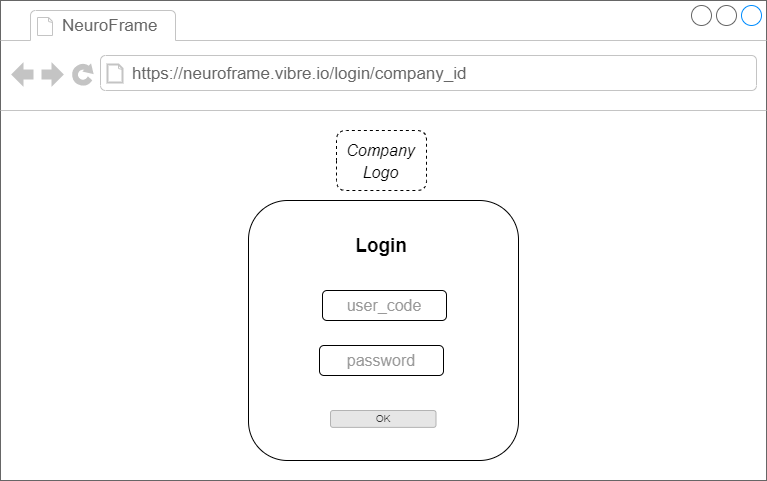
\includegraphics[width=0.85\textwidth]{img/wireframe_login.png}
  \caption{Pagina di login dell'applicativo Dashboard}
\end{figure}
\noindent Nel secondo wireframe possiamo individuare \emph{tre macro aree}:
\begin{itemize}
  \item \textbf{Impostazioni}\\
  In alto troviamo i componenti che permetteranno al Team manager di modificare varie impostazioni della visualizzazione a schermo e di gestire i componenti del team.
  \item \textbf{Area singoli componenti}\\
  Qui individuiamo i dati del benessere cognitivo relativi ad ogni componente del team.\newline
  I suddetti dati verranno mostrati al Team manager attraverso modalità di rappresentazione coerenti con il tipo di dato, ad esempio con grafici e labels.
  \item \textbf{Area del team}\\
  Quest'area risulta analoga alla visualizzazione dei dati di un singolo utente ma descrive il benessere del Team nel complesso.\newline
  Anche qui verranno utilizzate le stesse modalità di rappresentazione dei dati con aggiunta di label che descrivano dati di utilità (ad esempio il componente del Team più affaticato).
\end{itemize}
Analogamente alla schermata di login si vuole mostrare a schermo il logo dell'organizzazione fruitrice del servizio, affiancato al logo di Vibre.
\begin{figure}[H]
  \centering
  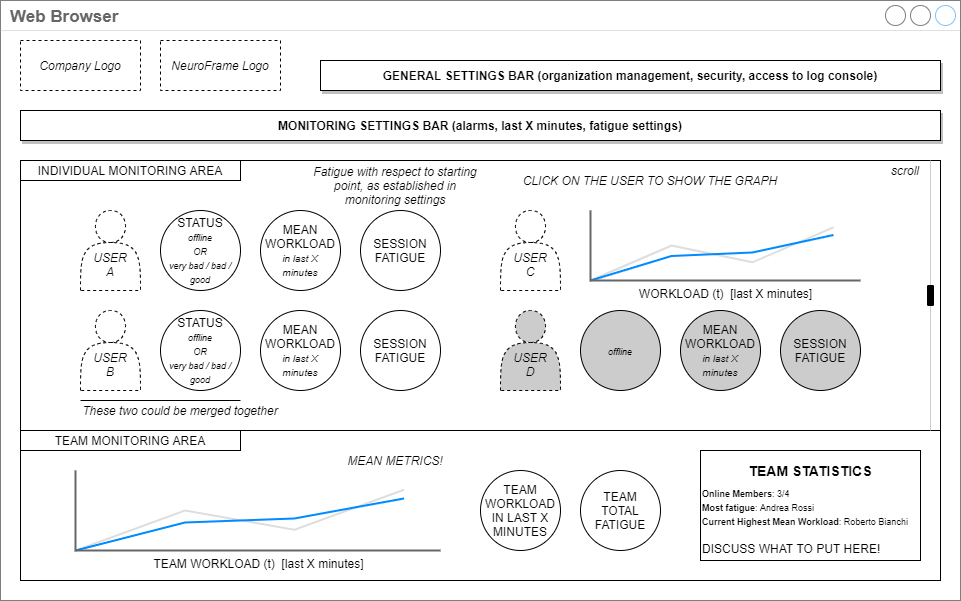
\includegraphics[width=0.9\textwidth]{img/wireframe_dashboard.png}
  \caption{Schermata Dashboard visualizzazione dati}
\end{figure}
\vspace{5mm}